%%%%%%%%%%%%%%%%%%%%%%%%%%%%% Define Article %%%%%%%%%%%%%%%%%%%%%%%%%%%%%%%%%%
\documentclass{article}   % two side printing
%%%%%%%%%%%%%%%%%%%%%%%%%%%%%%%%%%%%%%%%%%%%%%%%%%%%%%%%%%%%%%%%%%%%%%%%%%%%%%%

%%%%%%%%%%%%%%%%%%%%%%%%%%%%% Using Packages %%%%%%%%%%%%%%%%%%%%%%%%%%%%%%%%%%
\usepackage{geometry}
\usepackage{graphicx}
\usepackage{amssymb}
\usepackage{amsmath}
\usepackage{amsthm}
\usepackage{empheq}
\usepackage{mdframed}
\usepackage{booktabs}
\usepackage{lipsum}
\usepackage{color}
\usepackage{psfrag}
\usepackage{pgfplots}   % For plotting beautiful graphs
\usepackage{bm}
\usepackage[spanish]{babel}
\usepackage{biblatex} 
\usepackage{csquotes} 
\usepackage{setspace}
\usepackage{multicol}  
\usepackage[skip=3pt plus 1pt, indent=30pt]{parskip}    % Setting space between paragraphs and indent
\usepackage[T1]{fontenc}    % Output font encoding for international characters
\usepackage{helvet}        % Selecting font family
\usepackage{ragged2e}      % For text alignment
\usepackage{adjustbox}       % For defining new environments
\usepackage{siunitx}         % For SI units
\usepackage{fancyhdr}       % For defining headers and footers
\usepackage[cochineal]{newtxmath}
\usepackage{caption}
\usetikzlibrary{intersections}
\usetikzlibrary{decorations.text}
\usetikzlibrary{decorations.pathreplacing}
%%%%%%%%%%%%%%%%%%%%%%%%%%%%%%%%%%%%%%%%%%%%%%%%%%%%%%%%%%%%%%%%%%%%%%%%%%%%%%%

% Other Settings
\newcommand*{\freq}{\mathord{\mathit{f}}}
%\let\cleardoublepage=\clearpage
%\renewcommand{\baselinestretch}{1.5}
%%%%%%%%%%%%%%%%%%%%%%%%%% Page Setting %%%%%%%%%%%%%%%%%%%%%%%%%%%%%%%%%%%%%%%
\geometry{a4paper, textwidth=19cm, textheight=28.5cm, top=0.1cm, headheight=0.1cm}  % Setting page size
\graphicspath{{images/}}    % Setting path for images
\addbibresource{bibliography.bib}   % Setting path for bibliography
%%%%%%%%%%%%%%%%%%%%%%%%%% Define some useful colors %%%%%%%%%%%%%%%%%%%%%%%%%%
\definecolor{ocre}{RGB}{243,102,25}
\definecolor{mygray}{RGB}{243,243,244}
\definecolor{deepGreen}{RGB}{26,111,0}
\definecolor{shallowGreen}{RGB}{235,255,255}
\definecolor{deepBlue}{RGB}{61,124,222}
\definecolor{shallowBlue}{RGB}{235,249,255}
%%%%%%%%%%%%%%%%%%%%%%%%%%%%%%%%%%%%%%%%%%%%%%%%%%%%%%%%%%%%%%%%%%%%%%%%%%%%%%%

%%%%%%%%%%%%%%%%%%%%%%%%%% Define an orange box command %%%%%%%%%%%%%%%%%%%%%%%%
\newcommand\orangebox[1]{\fcolorbox{ocre}{mygray}{\hspace{1em}#1\hspace{1em}}}
%%%%%%%%%%%%%%%%%%%%%%%%%%%%%%%%%%%%%%%%%%%%%%%%%%%%%%%%%%%%%%%%%%%%%%%%%%%%%%%

%%%%%%%%%%%%%%%%%%%%%%%%%%%% English Environments %%%%%%%%%%%%%%%%%%%%%%%%%%%%%
\newtheoremstyle{mytheoremstyle}{3pt}{3pt}{\normalfont}{0cm}{\rmfamily\bfseries}{}{1em}{{\color{black}\thmname{#1}~\thmnumber{#2}}\thmnote{\,--\,#3}}
\newtheoremstyle{myproblemstyle}{3pt}{3pt}{\normalfont}{0cm}{\rmfamily\bfseries}{}{1em}{{\color{black}\thmname{#1}~\thmnumber{#2}}\thmnote{\,--\,#3}}
\theoremstyle{mytheoremstyle}
\newmdtheoremenv[linewidth=1pt,backgroundcolor=shallowGreen,linecolor=deepGreen,leftmargin=0pt,innerleftmargin=20pt,innerrightmargin=20pt,]{theorem}{Theorem}[section]
\theoremstyle{mytheoremstyle}
\newmdtheoremenv[linewidth=1pt,backgroundcolor=shallowBlue,linecolor=deepBlue,leftmargin=0pt,innerleftmargin=20pt,innerrightmargin=20pt,]{definition}{Definition}[section]
\theoremstyle{myproblemstyle}
\newmdtheoremenv[linecolor=black,leftmargin=0pt,innerleftmargin=10pt,innerrightmargin=10pt,]{problem}{Problem}[section]
%%%%%%%%%%%%%%%%%%%%%%%%%%%%%%%%%%%%%%%%%%%%%%%%%%%%%%%%%%%%%%%%%%%%%%%%%%%%%%%

%%%%%%%%%%%%%%%%%%%%%%%%%%%%%%% Plotting Settings %%%%%%%%%%%%%%%%%%%%%%%%%%%%%
\usepgfplotslibrary{colorbrewer}
\pgfplotsset{width=8cm,compat=1.9}
%%%%%%%%%%%%%%%%%%%%%%%%%%%%%%%%%%%%%%%%%%%%%%%%%%%%%%%%%%%%%%%%%%%%%%%%%%%%%%%

%%%%%%%%%%%%%%%%%%%%%%%%%%%%%%% Title & Author %%%%%%%%%%%%%%%%%%%%%%%%%%%%%%%%
\title{Determinación de la Constante de Propagación en Líneas de Transmisión mediante Análisis Matricial}
\author{Luis Guillermo Macias Rojas}
%%%%%%%%%%%%%%%%%%%%%%%%%%%%%%%%%%%%%%%%%%%%%%%%%%%%%%%%%%%%%%%%%%%%%%%%%%%%%%%

%%%%%%%%%%%%%%%%%%%%%%%%%%%%%%% Header & Footer %%%%%%%%%%%%%%%%%%%%%%%%%%%%%%%
\pagestyle{fancy}  % Setting page style
\fancyhf{}
\fancyhead[L]{\text{Luis Guillermo Macias Rojas}}  % Setting header
%%%%%%%%%%%%%%%%%%%%%%%%%%%%%%%%%%%%%%%%%%%%%%%%%%%%%%%%%%%%%%%%%%%%%%%%%%%%%%%

\begin{document}
    \maketitle

    \fontfamily{phv}\selectfont % Selecting font family
    \noindent
    \textbf{Resumen:} Este trabajo completa la caracterización de líneas de transmisión mediante: 1) Conversión de parámetros S a ABCD 
    para obtener $Z_c$, 2) Cálculo de $C$ y $L$ a partir del producto $\gamma Z_c$ (parte real e imaginaria respectivamente), 3) Determinación de $R$ y $G$ mediante ADS, y 4) 
    Validación con modelo distribuido de $N$ etapas. Los resultados muestran que 32 etapas son suficientes para que el error entre las 
    mediciones del VNA y los obtenidos por el modelo distribuido sea mínimo.

    \noindent\begin{minipage}{0.49\textwidth}   %uses 60% of the page
        {\centering\section*{\large Introducción}}

        Partiendo del trabajo previo donde se obtiene $\gamma$ mediante el metodo unificado, se procede a calcular $Z_c$ utilizando la 
        ecuación \eqref{eq:Zc_ABCD}; la cual se deriva de la relación entre los parámetros S y ABCD.
        
        \begin{equation}
            Z_c = \sqrt{\frac{B}{C}}
            \label{eq:Zc_ABCD}
        \end{equation}

        $Z_c$ es la impedancia característica de la línea de transmisión, que se relaciona con la constante de propagación $\gamma$ a través de la ecuación \eqref{eq:gamma_Zc}.
        \begin{equation}
            \gamma = \frac{1}{Z_c}\left(R + j\omega L\right)
            \label{eq:gamma_Zc}
        \end{equation}

        {\centering\section*{\large Metodología}}

        Obteniendo $Z_c$ de la ecuación \eqref{eq:Zc_ABCD}, se procede a calcular $C$ y $L$ a partir del producto $\gamma Z_c$.
        La relación entre C la parte real de $Z_c$ está dada por la ecuación \eqref{eq:Zc_C}, donde el valor aproximado de Re($Z_c$)
        es de 60 $\Omega$ según simulaciones de ADS.

        \begin{equation}
            C = \frac{\beta}{Re(Z_c) \cdot \omega} \approx 80 \, \text{pF}
            \label{eq:Zc_C}
        \end{equation}

        Para calcular $L_{\infty}$ se utiliza la ecuación \eqref{eq:Zc_L}, donde el valor de $K_s \approx 0.0006$ como sugiere la Figura
        \ref{fig:K_s}.
        \begin{equation}
            L_{\infty} = L - \frac{K_s}{2\pi \sqrt{f}} \approx 0.3 \, \mu H
            \label{eq:Zc_L}
        \end{equation}

        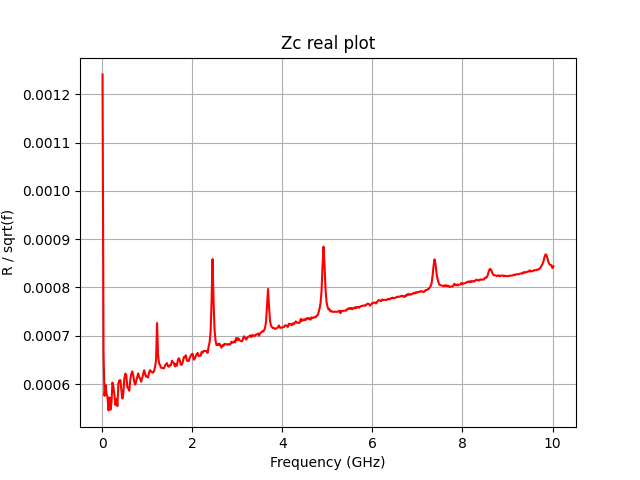
\includegraphics[width=\textwidth]{figures/ks_plot.png}
        \captionof{figure}{Gráfica de $\frac{K_s}{\sqrt{f}}$ vs $f$ para determinar el valor de $K_s$.}
        \label{fig:K_s}


    \end{minipage}
    \hspace{0.38 cm}
    \begin{minipage}{0.49\textwidth}   %uses 40% of the page
        Por último, se obtiene $R$ y $G$ en ADS y se determina de manera heurística el número de 
        etapas mínimo para que los resultados sean similares a los medidos por el VNA.
        
        {\centering\section*{\large Resultados}}
        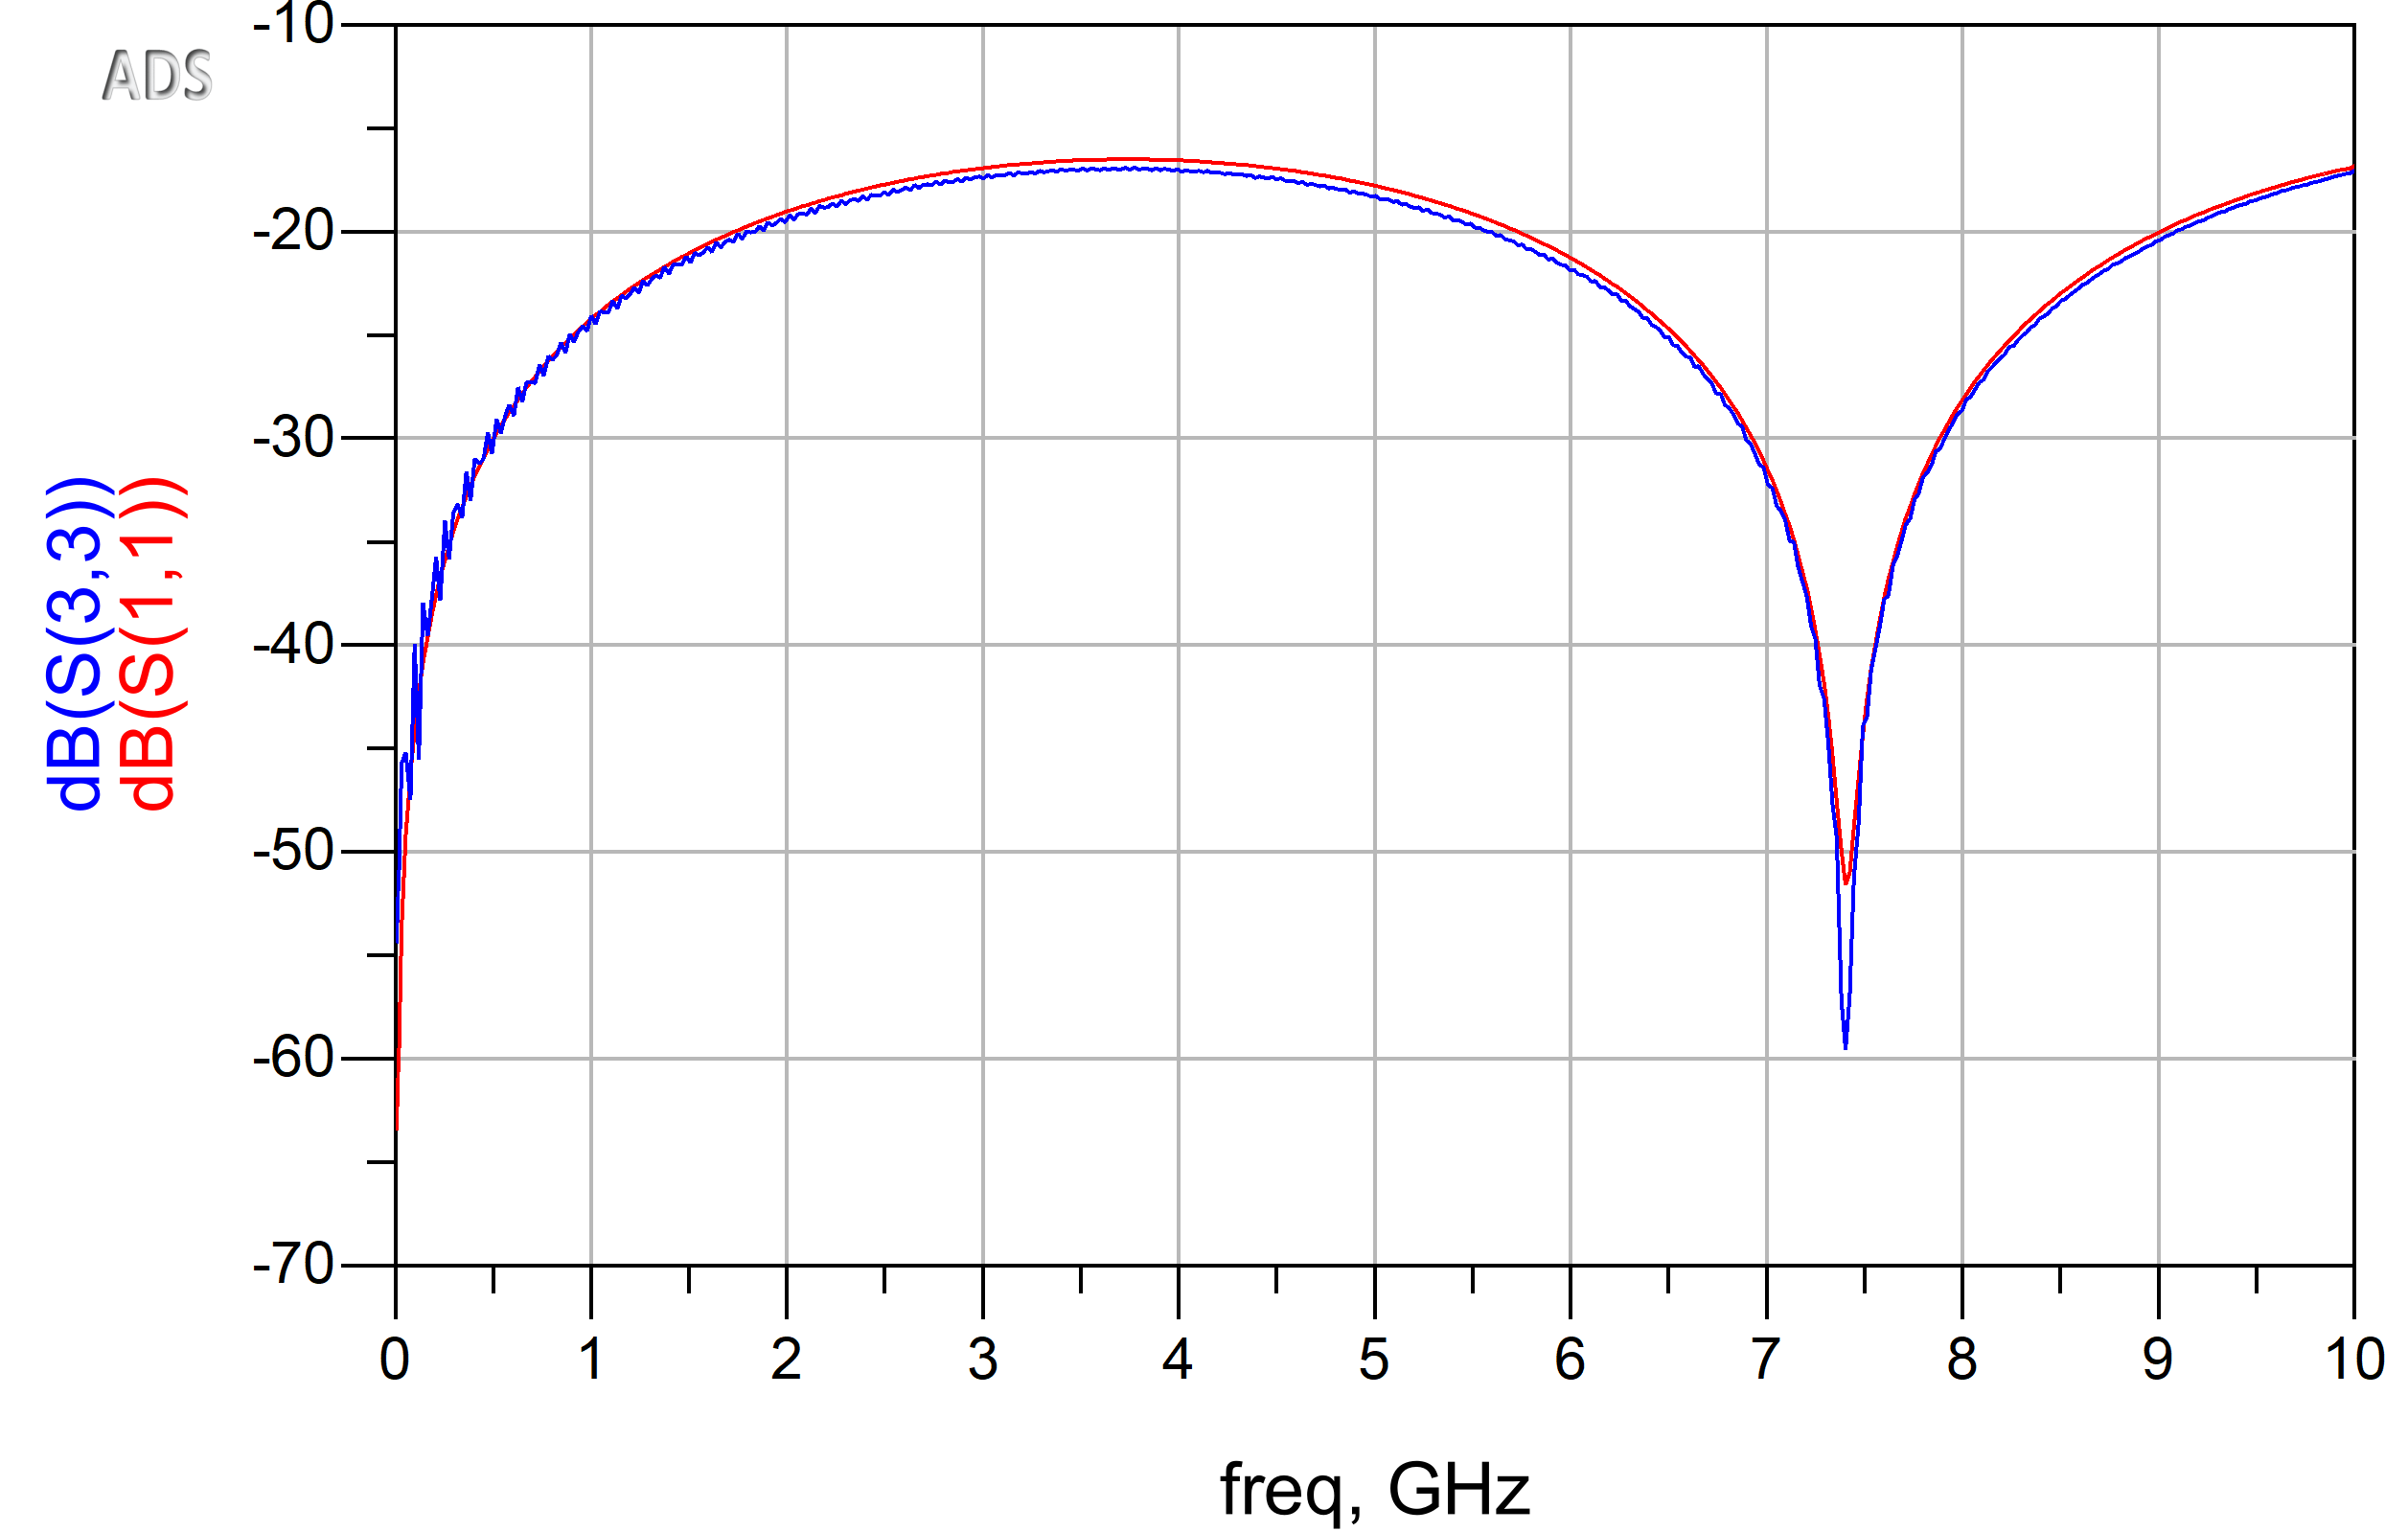
\includegraphics[width=\textwidth]{figures/magnitud_s11.png}
        \captionof{figure}{Reflexión (S$_{11}$) de línea de transmisión de 0.5": VNA (azul), modelo de 32 etapas (rojo).}
        \label{fig:gamma_real}
        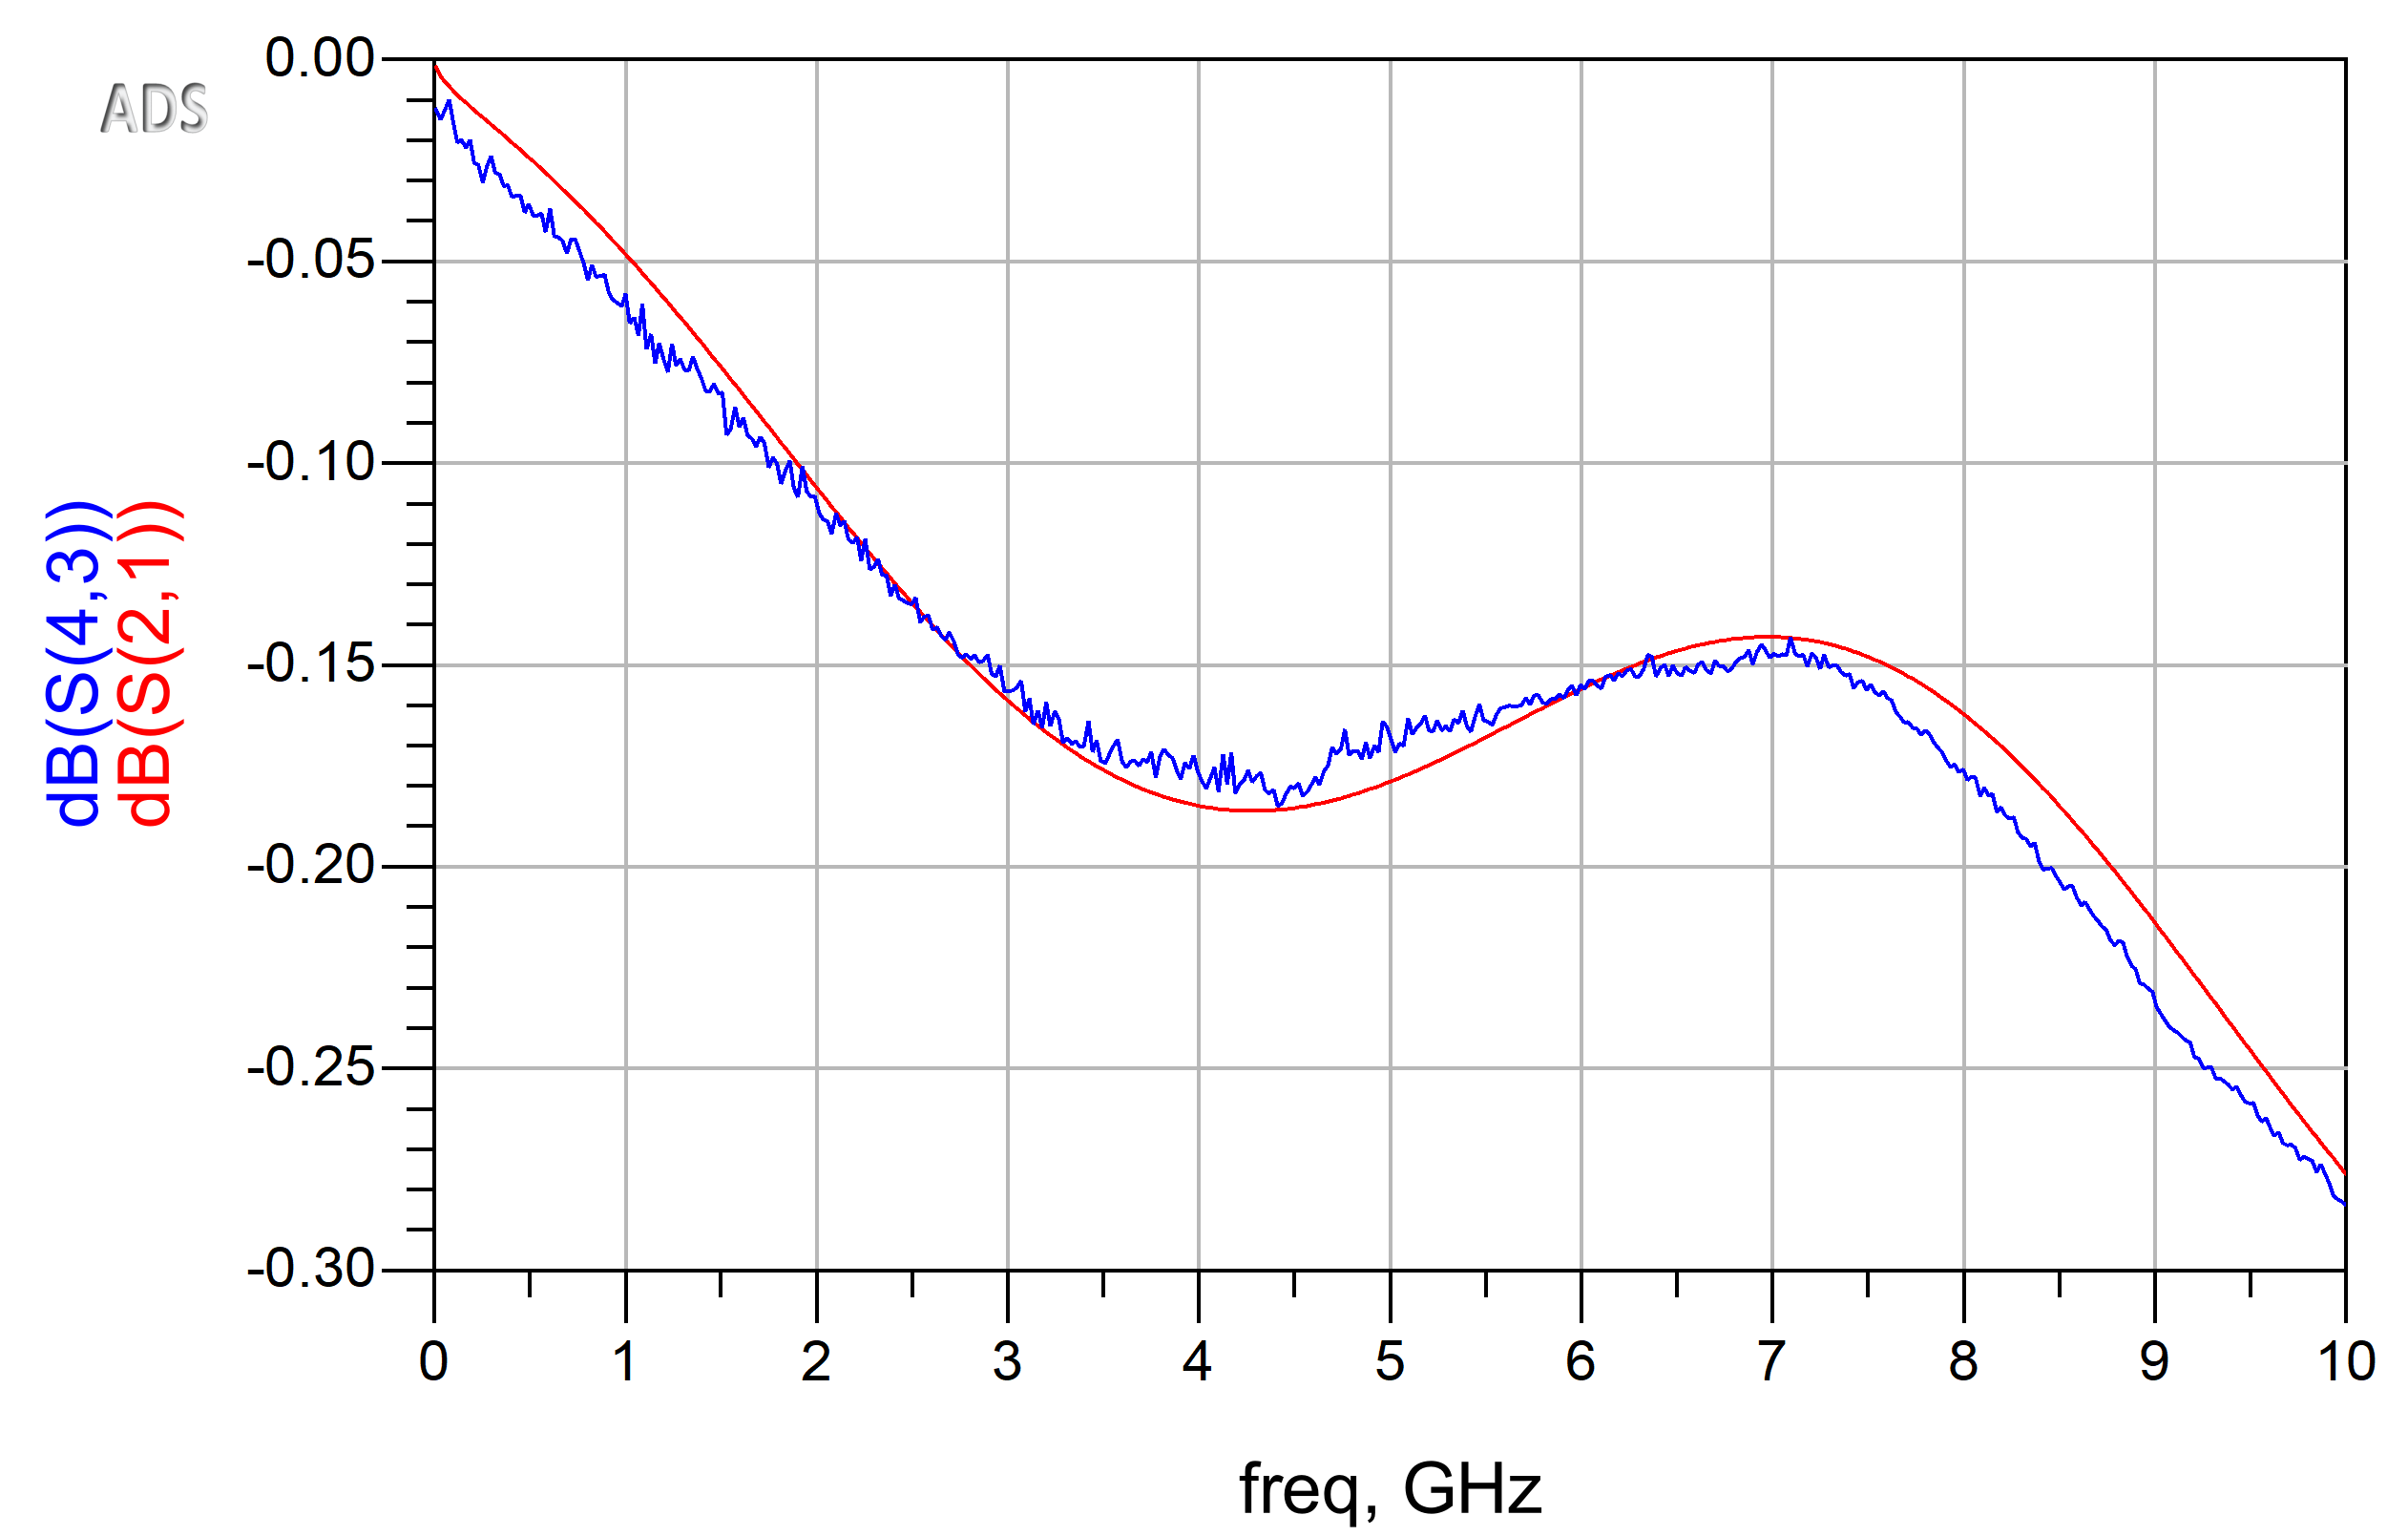
\includegraphics[width=\textwidth]{figures/s21_tarea6.png}
        \captionof{figure}{Transmisión (S$_{21}$) de línea de transmisión de 0.5": VNA (azul), modelo de 32 etapas (rojo).}
        \label{fig:gamma_imag}

        {\centering\section*{\large Conclusiones}}
        El modelo distribuido resulta en una buena aproximación a la línea de transmisión. Se concluye que 32 etapas son suficientes para 
        que el error entre las mediciones del VNA y los obtenidos por el modelo distribuido sea mínimo. Las aproximaciones de las ecuaciones
        \eqref{eq:Zc_C} y \eqref{eq:Zc_L} son válidas, pero requieren un ajuste fino heurístico para obtener resultados precisos.
        %\printbibliography  % Print bibliography
    \end{minipage}
\end{document}